\chapter{VsCode 配置python}
\section{安装Python插件}
刚刚安装成功的 VS Code 是没有 Python 扩展的在欢迎界面中选择 "Python"，下方会弹出一个对话框，选择 "OK"，即可完成 Python 扩展的
安装；
\begin{figure}[htpb]
    \centering
    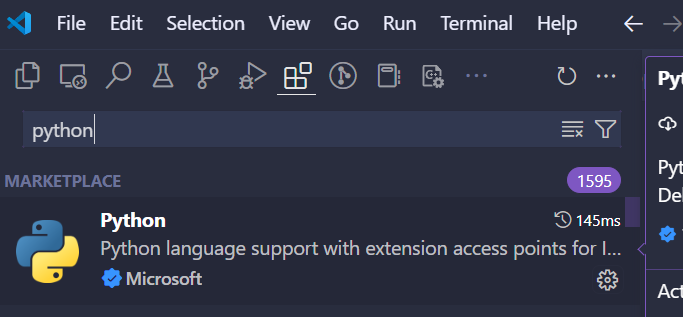
\includegraphics[width=0.6\textwidth]{part/软件工程/环境搭建/IDE/pic/VSCode/python插件.png}
    \caption{VsCode 安装Python插件}
\end{figure}

